% Chapter Template

\chapter{Question 3} % Main chapter title

\label{Question 3} % Change X to a consecutive number; for referencing this chapter elsewhere, use \ref{ChapterX}

\lhead{ \emph{EXT 4}} % Change X to a consecutive number; this is for the header on each page - perhaps a shortened title

%----------------------------------------------------------------------------------------
%	SECTION 1
%----------------------------------------------------------------------------------------
\section{Performances de EXT4}
Pour démarrer cet exercice, il est important de prendre connaissance de la page de manuel de la commande mount qui donne ceci:
\begin{lstlisting}[style=Bash]
data={journal|ordered|writeback}
              Specifies the journalling mode for file data.  Metadata is always journaled.  To use modes other than ordered on the root filesystem, pass the mode to the kernel  as  boot  parameter,  e.g.
              rootflags=data=journal.

              journal
                     All data is committed into the journal prior to being written into the main filesystem.

              ordered
                     This is the default mode.  All data is forced directly out to the main file system prior to its metadata being committed to the journal.

              writeback
                     Data  ordering  is  not  preserved - data may be written into the main filesystem after its metadata has been committed to the journal.  This is rumoured to be the highest-throughput
                     option.  It guarantees internal filesystem integrity, however it can allow old data to appear in files after a crash and journal recovery.

       barrier=0 / barrier=1
              This enables/disables barriers.  barrier=0 disables it, barrier=1 enables it.  Write barriers enforce proper on-disk ordering of journal commits, making volatile disk write caches  safe  to
              use,  at some performance penalty.  The ext3 filesystem does not enable write barriers by default.  Be sure to enable barriers unless your disks are battery-backed one way or another.  Oth‐
              erwise you risk filesystem corruption in case of power failure.
\end{lstlisting}

De plus, il a été préalablement nécessaire d'installer un cross-compilateur pour Odroid sur la machine hôte utilisée. Ainsi, l'installation a été réalisée à l'aide des commandes suivantes:
\begin{lstlisting}[style=Bash]
cd /usr/local/arm
wget https://launchpadlibrarian.net/129963014/gcc-linaro-arm-linux-gnueabihf-4.7-2013.01-20130125_linux.tar.xz
xz -d gcc-linaro-arm-linux-gnueabihf-4.7-2013.01-20130125_linux.tar.xz 
tar -xvf gcc-linaro-arm-linux-gnueabihf-4.7-2013.01-20130125_linux.tar
ln -s gcc-linaro-arm-linux-gnueabihf-4.7-2013.01-20130125_linux /usr/local/arm/toolchain
\end{lstlisting}
Cette installation a permis de compiler le logiciel permettant de réaliser les mesures sur la copie des fichiers. En effet, Linux propose la fonction \textbf{date} qui peut-être utilisée pour récupérer un timestamp temporel mais sur le système embarqué, cette commande n'a pas pu fournir la précision à la milliseconde. Ainsi, il a été nécessaire d'écrire et exécuter un programme le permettant. Le code de ce programme est donné en listing \ref{lst:measure copy time}. Le makefile permettant de le compiler est donné en listing \ref{lst:makefile ext4}. De plus, afin de simplifier les tests de fonctionnement, le code a d'abord été compilé pour la machine hôte.
\begin{lstlisting}[language=C,caption=Mesure du temps de copie,label=lst:measure copy time]
#include <ctime>
#include <iostream>
#include <fstream>

using namespace std;

int main (int argc, char * argv[])
{
	if (argc > 0)
	{
		ifstream srcFile (argv[1], ios::binary);
		ofstream dstFile ((string(argv[2]) + string("copy-of-") + string(argv[1])).c_str(), ios::binary);
		
		clock_t	begin = clock();
		dstFile << srcFile.rdbuf();
		clock_t	end = clock();
		
		dstFile.close();
		srcFile.close();
		
		// Returns time in microseconds
		cout << ((double)(end - begin) / (CLOCKS_PER_SEC / 1000000.));
	}
	
	return 0;
}
\end{lstlisting}
\begin{lstlisting}[label=lst:makefile ext4,caption=makefile permettant la compilation pour la cible]
CROSS_COMPILE_PATH=/usr/local/arm/toolchain/bin
ARCH=arm
CROSS_COMPILE=arm-linux-gnueabihf-
CC=$(CROSS_COMPILE)g++
CXXFLAGS=-m$(ARCH) -mthumb-interwork -W -Wall

EXEC=copyFile
EXT=cpp
LDFLAGS=

all: $(EXEC)

copyFile: $(EXEC).o 
	PATH=$(PATH):$(CROSS_COMPILE_PATH)
	$(CC) -o $@ $^ $(LDFLAGS)

%.o: %.$(EXT)
	PATH=$(PATH):$(CROSS_COMPILE_PATH)
	$(CC) -o $@ -c $< $(CXXFLAGS)

clean:
	rm -rf *.o
	rm -f $(EXEC)
\end{lstlisting}

Une fois le fichier binaire compilé, un script permettant la mesure automatique des performances des différentes options sur le EXT4 a été rédigé. Ce script mesure le temps de copie d'un fichier de 50MB et d'un fichier de 50kB avec les options de \textbf{journalisation}, \textbf{data=journal}, \textbf{data=ordered}, \textbf{data=writeback}, \textbf{barrier=0} et \textbf{barrier=1}. Les résultats sont donnés ci-dessous.
\begin{lstlisting}
#!/bin/sh

#
# FUNCTIONS
#
backupFstab () {
	cp /etc/fstab ./fstab
	cp /etc/fstab /etc/fstab.bck
}
restoreFstab () {
	cp ./fstab /etc/fstab
}
createFiles () {
	echo -n "Creating the file bigFile ... "

	# Create the file
	ddResult=$(dd if=/dev/urandom of=./bigFile bs=${S_SIZE} count=$((BIG_SIZE / S_SIZE)) 2>&1)
	echo -e "[ \e[92mOK\e[0m ]"
	echo $ddResult

	echo -n "Creating the file smallFile ... "
	
	# Create the file
	ddResult=$(dd if=/dev/urandom of=./smallFile bs=${S_SIZE} count=$((SMALL_SIZE / S_SIZE)) 2>&1)
	echo -e "[ \e[92mOK\e[0m ]"
	echo $ddResult
}

journaling () {
	echo "Un mounting "${TARGET_DIR}
	umount ${TARGET_DIR}
	if [[ $1 -eq 0 ]]; then
		echo "Disabling journal on /dev/mmcblk0p3"
		tune2fs -O ^has_journal /dev/mmcblk0p3
	else
		echo "Enabling journal on /dev/mmcblk0p3"
		tune2fs -O has_journal /dev/mmcblk0p3
	fi

	# Mounting partition
	echo "Re mount "${TARGET_DIR}
	mount -t ext4 /dev/mmcblk0p3 ${TARGET_DIR}
}

mountOptions () {
	# Mount usrfs partition
	echo -n "changing "$1" option on /dev/mmcblk0p3"
	umount /dev/mmcblk0p3
	cp ./fstabFiles/fstab-${1} /etc/fstab
	mount /dev/mmcblk0p3
	echo "[ OK ]"
}

run () {
	echo "Starting measure ..."
	./measure ${RESULTS_FILE} ${TARGET_DIR}
}

removeFiles () {
	echo "Removing bigFile ... "
	rm -f bigFile 
	rm -f smallFile
}

# Big file size
BIG_SIZE=50000000

# Small file size
SMALL_SIZE=50000

# Bloc sector size
S_SIZE=512

# Results file
RESULTS_FILE=results.txt
TARGET_DIR=/mnt/usr

backupFstab
createFiles

#
# Disable journaling
#
journaling 0
run

#
# Enables journaling
#
journaling 1
run

#
# data journal option
#
mountOptions data-journal
run

mountOptions data-ordered
run

mountOptions data-writeback
run

mountOptions barrier-1
run

mountOptions barrier-0
run

restoreFstab
removeFiles
\end{lstlisting}

\subsection{Mesures}
Les résultats de ces mesures sont données par la figure \ref{fig:measure ext4}.
\begin{figure}[H]
	\centering
	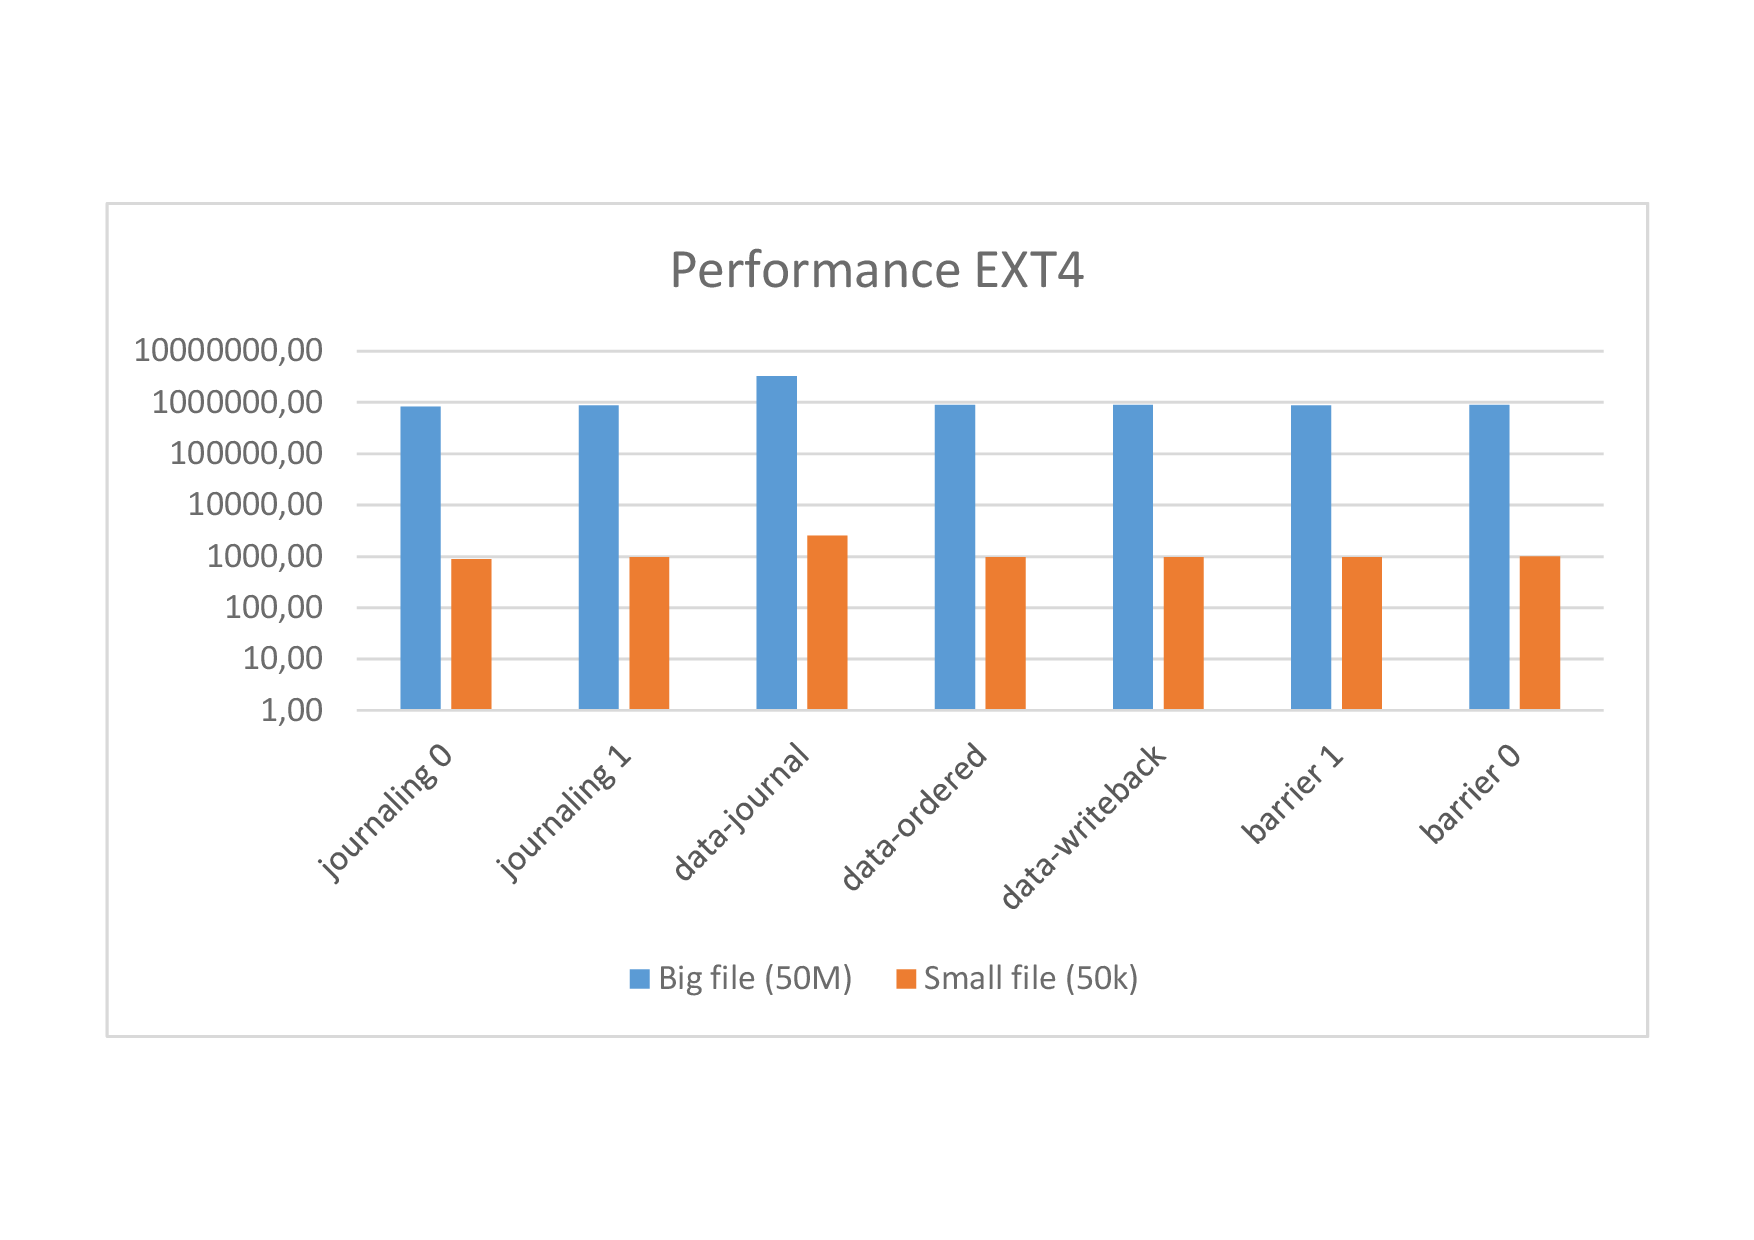
\includegraphics[width=14cm]{ext4/measures.png}
	\caption{\label{fig:measure ext4}Résultats de mesure sur EXT4}
\end{figure}

De ces résultats il vient que l'option qui ralenti le plus le système de fichier est la journalisation. Toute les autres options restent très proches les unes des autres en terme de performance. Dans le graphique \ref{fig:measure ext4}, une échelle logarithmique a été utilisée pour faciliter la lecture des données. De plus, il n'a pas été jugé pertinent de fournir un graphe détaillé des différents temps car ceux-ci varient de $\pm 100\ ms$ et restent sous la barre des 970 ms d'une option à l'autre pour un fichier de 50 MB.

La journalisation des données prend plus de temps car le système garde une trace de ce qui a été modifié.

Pour cet exercice il a fallu au préalable installer et compiler l'application \textbf{tune2fs} à l'aide de buildroot.

\section{SquashFS}
Le système de fichier Squash est un système de type lecture-seule et supportant la compression. Il supporte des tailles de blocs jusqu'à 1Mo afin d'optimiser la compression des fichiers. Pour pouvoir l'utiliser sous Linux, il est au préalable nécessaire de modifier la compilation du kernel afin de le lui faire supporter. Ainsi, l'exécution et la configuration sont données:

\begin{lstlisting}
make linux-menuconfig
    File systems  --->
[*] Miscellaneous filesystems  --->
<*>   SquashFS 4.0 - Squashed file system support
\end{lstlisting}

Afin de réaliser correctement cet exercice, quatre images squashFS ont été créées à l'aide des fichiers et dossiers générés par buildroot lors de la compilation du Kernel. Le script permettant la création des images est donné ci-dessous \ref{lst:squashfs}. Les images obtenues ainsi que leur taille respectives sont données dans le tableau ci-dessous:
\begin{table}[H]
	\centering
	\begin{tabular}{lrp{10cm}}
	Fichier & Taille [ko] & Description\\
	squashfs.default & 14487.5 & image squashfs sans option de compression\\
	squashfs.noD & 26771.4 & image squashfs sans compression des blocs de données\\
	squashfs.noI & 14553.1 & image squashfs sans compression de la table des i-noeuds\\
	squashfs.noF & 24772.6 & image squashfs sans compression des blocs fragmentés
	\end{tabular}
	\caption{\label{table:squashfs size}Résumé de la taille de chaque image squashfs}
\end{table}

\begin{lstlisting}[caption=Création des images squash fs,label=lst:squashfs]
#!/bin/bash

TARGET_DIR=/media/embedhfw/usrfs
BUILDROOT_ROOTFS=~/ses/buildroot/output/images

if [[ ! -d "$TARGET_DIR" ]];
then
	echo $TARGET_DIR" is not mounted, please mount it first."
	echo "Quit"
	exit
fi

# File system is mounted

mkdir tmpfs
echo "mounting rootfs.ext4 from buildroot/output/images"
mount -t ext4 ${BUILDROOT_ROOTFS}/rootfs.ext4 ./tmpfs

echo "Copy specified folders to $TARGET_DIR"
cp -R tmpfs/{bin,lib,lib32,libexec,sbin,share} $TARGET_DIR

echo "Creating squash fs file with default parameters"
mksquashfs tmpfs squashfs.default

echo "Creating squash fs file without inode compression"
mksquashfs tmpfs squashfs.noI -noI

echo "Creating squash fs file without data compression"
mksquashfs tmpfs squashfs.noD -noD

echo "Creating squash fs file without fragment compression"
mksquashfs tmpfs squashfs.noF -noF

umount ./tmpfs
\end{lstlisting}

Les images du système de fichier \textbf{squash} créées, celle par défaut (squashsf.default) a été montée dans \textbf{/mnt/sqfs} afin de réaliser quelques tests d'écriture.
\begin{lstlisting}[style=Bash]
# pwd
/mnt/sqfs
# mount squashfs.default /mnt/sqfs -t squashfs -o loop
# mount
rootfs on / type rootfs (rw)
/dev/root on / type ext4 (rw,relatime,data=ordered)
devtmpfs on /dev type devtmpfs (rw,relatime,size=765120k,nr_inodes=120929,mode=755)
proc on /proc type proc (rw,relatime)
devpts on /dev/pts type devpts (rw,relatime,gid=5,mode=620)
tmpfs on /dev/shm type tmpfs (rw,relatime,mode=777)
tmpfs on /tmp type tmpfs (rw,relatime)
sysfs on /sys type sysfs (rw,relatime)
/dev/mmcblk0p3 on /mnt/usr type ext4 (rw,relatime,data=ordered)
/dev/loop0 on /mnt/sqfs type squashfs (ro,relatime)
# ls -la /mnt/sqfs
total 1
drwxr-xr-x   18 root     root           256 Apr 30  2015 .
drwxr-xr-x    4 root     root          1024 Jan  1 00:02 ..
drwxrwxr-x    2 root     root           993 Apr 30  2015 bin
drwxr-xr-x    3 root     root            52 Apr 14  2015 dev
drwxr-xr-x    7 root     root           439 Apr 30  2015 etc
drwxrwxr-x    3 root     root            26 Mar  5  2015 home
drwxrwxr-x    5 root     root           953 Apr 30  2015 lib
lrwxrwxrwx    1 root     root             3 Apr 14  2015 lib32 -> lib
lrwxrwxrwx    1 root     root            11 Apr 14  2015 linuxrc -> bin/busybox
drwx------    2 root     root             3 Apr 30  2015 lost+found
drwxrwxr-x    2 root     root             3 Mar  5  2015 media
drwxrwxr-x    2 root     root             3 Feb  3  2015 mnt
drwxrwxr-x    2 root     root             3 Feb  3  2015 opt
drwxrwxr-x    2 root     root             3 Feb  3  2015 proc
drwx------    2 root     root            77 Mar  5  2015 root
drwxrwxr-x    2 root     root           744 Apr 30  2015 sbin
drwxrwxr-x    2 root     root             3 Mar  5  2015 sys
drwxrwxrwt    2 root     root             3 Feb  3  2015 tmp
drwxrwxr-x    7 root     root           102 Apr 30  2015 usr
drwxrwxr-x    6 root     root            63 Apr 14  2015 var
# mkdir /mnt/sqfs/test
mkdir: can't create directory '/mnt/sqfs/test': Read-only file system
\end{lstlisting}

Le listing ci-dessus illustre clairement qu'il n'a pas été possible de créer un dossier dans l'arborescence du système de fichier. Le même test a été réalisé pour chaque cas. Mêmes résultats, donnés par le listing \ref{lst:squash nod}

\begin{lstlisting}[style=Bash,caption=squashfs.noD,label=squash nod]
# mount squashfs.noD /mnt/sqfs -t squashfs -o loop
# mkdir /mnt/sqfs/test
mkdir: can't create directory '/mnt/sqfs/test': Read-only file system
# mount squashfs.noF /mnt/sqfs -t squashfs -o loop
# mkdir /mnt/sqfs/test
mkdir: can't create directory '/mnt/sqfs/test': Read-only file system
# mount squashfs.noI /mnt/sqfs -t squashfs -o loop
# mkdir /mnt/sqfs/test
mkdir: can't create directory '/mnt/sqfs/test': Read-only file system
\end{lstlisting}

\section{Partition squashfs}
Pour réaliser cet exercice, un script de création de la carte SD a été exécuté lorsque la carte \usd se trouvait dans le lecteur. Le système cible à ensuite pu être démarré. Après avoir modifié le contenu du fichier /etc/fstab tel que donné ci-dessous
\begin{lstlisting}
# /etc/fstab: static file system information.
#
# <file system> <mount pt>     <type>   <options>         <dump> <pass>
/dev/root       /              ext2     rw,noauto         0      1
proc            /proc          proc     defaults          0      0
devpts          /dev/pts       devpts   defaults,gid=5,mode=620   0      0
tmpfs           /dev/shm       tmpfs    mode=0777         0      0
tmpfs           /tmp           tmpfs    mode=1777         0      0
sysfs           /sys           sysfs    defaults          0      0
/dev/mmcblk0p3  /mnt/usr       ext4     defaults          0      0
/dev/mmcblk0p4  /mnt/sqfs      squashfs defaults          0      0
\end{lstlisting}

les partitions ont pu être montées après création de leur point de montage sur la partition \textbf{rootfs}.
\begin{lstlisting}
# mkdir /mnt/usr
# mkdir /mnt/sqfs
\end{lstlisting}

Ainsi, le montage du système de fichier \textbf{squashfs} donne les résultats suivants :
\begin{lstlisting}[style=Bash]
# mount -a
[  110.733993] [c7] EXT4-fs (mmcblk0p3): mounted filesystem with ordered data mode. Opts: (null)
Jan  1 00:52:27 odroidxu3 user.info kernel: [  110.733993] [c7] EXT4-fs (mmcblk0p3): mounted filesystem with ordered data mode. Opts: (null)
# ls /mnt/usr/
lost+found
# ls /mnt/sqfs/
bin         home        linuxrc     mnt         root        tmp
dev         lib         lost+found  opt         sbin        usr
etc         lib32       media       proc        sys         var
# mount
rootfs on / type rootfs (rw)
/dev/root on / type ext4 (rw,relatime,data=ordered)
devtmpfs on /dev type devtmpfs (rw,relatime,size=765120k,nr_inodes=120929,mode=755)
proc on /proc type proc (rw,relatime)
devpts on /dev/pts type devpts (rw,relatime,gid=5,mode=620)
tmpfs on /dev/shm type tmpfs (rw,relatime,mode=777)
tmpfs on /tmp type tmpfs (rw,relatime)
sysfs on /sys type sysfs (rw,relatime)
/dev/mmcblk0p3 on /mnt/usr type ext4 (rw,relatime,data=ordered)
/dev/mmcblk0p4 on /mnt/sqfs type squashfs (ro,relatime)
\end{lstlisting}

\subsection{Vérification de lecture seule}
Un premier test de lecture seule a été réalisé à l'aide de la commande mkdir qui permet de créer un dossier. Cette commande a échoué sur le système de fichier cible (/mnt/sqfs:squashfs) qui signale "\textbf{Read-only file system}".
\begin{lstlisting}
# mkdir /mnt/sqfs/test
mkdir: can't create directory '/mnt/sqfs/test': Read-only file system
\end{lstlisting}

Un second test a été réalisé à l'aide de l'édition du fichier \textbf{/etc/fstab} se trouvant sur le système cible. Le logiciel \textbf{vi} signale
\begin{lstlisting}[style=Bash]
- etc/fstab [Readonly] 1/9 11%
\end{lstlisting}
lors de l'édition. Le test a ensuite été poursuivi lors de la modification de ce fichier puis de sa sauvegarde. En effet, vi signale
\begin{lstlisting}[style=Bash]
'etc/fstab' is read only
\end{lstlisting}
lors de la commande
\begin{lstlisting}[style=Bash]
:wq
\end{lstlisting}
exécutée dans \textbf{vi}. Le système de fichier squashfs est effectivement en lecture seule et ne permet donc pas l'écriture ou la création de nouveaux fichiers.
